\documentclass{article}
\usepackage[utf8]{inputenc} % allow utf-8 input
\usepackage[T1]{fontenc}    % use 8-bit T1 fonts
\usepackage{hyperref}       % hyperlinks
\usepackage{url}            % simple URL typesetting
\usepackage{booktabs}       % professional-quality tables
\usepackage{amsfonts}       % blackboard math symbols
\usepackage{nicefrac}       % compact symbols for 1/2, etc.
\usepackage{microtype}      % microtypography

\usepackage[english]{babel}
\usepackage{blindtext}
\usepackage{bm}
\usepackage{index}
\usepackage[utf8]{inputenc}
\usepackage{graphicx}
\graphicspath{ {./} }
\usepackage{amsmath}
\usepackage{amssymb}
\usepackage{listings}
\usepackage{color}
\usepackage{siunitx}
\usepackage{longtable}

\definecolor{dkgreen}{rgb}{0,0.6,0}
\definecolor{gray}{rgb}{0.5,0.5,0.5}
\definecolor{mauve}{rgb}{0.58,0,0.82}

\lstset{frame=tb,
  language=Python,
  aboveskip=3mm,
  belowskip=3mm,
  showstringspaces=false,
  columns=flexible,
  basicstyle={\small\ttfamily},
  numbers=none,
  numberstyle=\tiny\color{gray},
  keywordstyle=\color{blue},
  commentstyle=\color{dkgreen},
  stringstyle=\color{mauve},
  breaklines=true,
  breakatwhitespace=true,
  tabsize=3
}
%% ========New command added by Han Liu===========================
\renewcommand{\vec}[1]{\boldsymbol{#1}}
\newenvironment{qparts}{\begin{enumerate}[1.]}{\end{enumerate}}
\usepackage{amsmath,textcomp,amssymb,geometry,graphicx,enumerate}
\usepackage{subcaption}
\usepackage[figurename=Fig.,labelfont=bf,labelsep=period]{caption}
\usepackage[capitalise]{cleveref}
\usepackage[ruled,vlined]{algorithm2e}
%% ===============================================================

\begin{document}
\title{EECS289A Introduction to Machine Learning,  Project T Final - Quiz Questions}
\author{%
  \ Han Liu, \ Peng Tan, \ Dilu Xu, \ Jinyan Zhao \\
  Department of Civil Engineering\\
  Universitu of California, Berkeley\\
  Berkeley, CA 94704 \\
  \texttt{\{han\_liu, tanpeng, diluxu, jinyan\_zhao\}@berkeley.edu} \\
}
\maketitle

\section{Elastic Net (HL)}
In class we discussed two types of regularization, $l_1$ and $l_2$. Both are useful, and sometimes it is helpful combine them, giving the objective function below (\textbf{in this problem we have excluded} $w_0$ \textbf{for simplicity}):
\begin{equation}
F(\vec{w}) = \frac{1}{2}\sum^n_{j=1}(y^{(j)}-\sum^d_{i=1}\vec{w}_i\vec{x}_i^{(j)})^2+\alpha\sum^d_{i=1}|\vec{w}_i|+\frac{\lambda}{2}+\sum^d_{i=1}\vec{w}_i^2
\end{equation}
Here, $(\vec{x}^{(j)},y^{(j)})$ is j-th example in the training data, w is a d dimensional weight vector, $\lambda$ is a regularization parameter for the $l_2$ norm of w, and $\alpha$ is a regularization parameter for the $l_1$ norm of w. This approach is called the Elastic Net, and you can see that it is a generalization of Ridge and Lasso regression: It reverts to Lasso when $\lambda = 0$, and it reverts to Ridge when $\alpha = 0$. In this question, we are going to derive the coordinate descent (CD) update rule for this objective.

Let g, h, c be real constants, and consider the function of x
\begin{equation}
f_1(x) = c+gx+\frac{1}{2}hx^2
\end{equation}
\begin{qparts}
\item {[}4 points{]} 
What is the $x^*$ that minimizes $f_1(x)$? (i.e. calculate $x^*=\arg\min f_1(x)$)\\
\underline{\textbf{Answer:}}\\
Take the gradient of $f_1(x)$ and set it to 0.
\begin{alignat}{2}
g+hx&=0 \\
x^*&=-\frac{g}{h}
\end{alignat}   

Let $\alpha$ be an additional real constant, and consider another function of x
\begin{equation}\label{eq:hl1}
f_2(x) = c+gx+\frac{1}{2}hx^2+\alpha|x|(h>0, \alpha>0)
\end{equation}
This is a piecewise function, composed of two quadratic functions:
\begin{equation}
f_2^-(x) = c+gx+\frac{1}{2}hx^2-\alpha x
\end{equation}
and
\begin{equation}
f_2^+(x) = c+gx+\frac{1}{2}hx^2+\alpha x
\end{equation}
Let $\tilde{x}^-=\arg\min_{x\in\mathbb{R}}f_2^-(x)$ and $\tilde{x}^+=\arg\min_{x\in\mathbb{R}}f_2^+(x)$.\\
(\textbf{Note:} The argmin is taken over $(-\infty, +\infty)$ here.
\\

\item {[}6 points{]} 
What are $\tilde{x}^+$ and $\tilde{x}^+$? Show that $\tilde{x}^-\geq\tilde{x}^+$. \\
\underline{\textbf{Answer:}}\\
Using the answer from part 1), we get $\tilde{x}^+=-\frac{g+\alpha}{h}$ and $\tilde{x}^-=-\frac{g-\alpha}{h}$. Since $\tilde{x}^--\tilde{x}^+=\frac{2\alpha}{h}\geq 0$, we have $\tilde{x}^-\geq\tilde{x}^+$.


\item {[}12 points{]} 
Draw a picture of $f_2(x)$ in each of the three cases below:
\begin{enumerate}[(a)]
\item $\tilde{x}^->0$, $\tilde{x}^+>0$
\item $\tilde{x}^-<0$, $\tilde{x}^+<0$
\item $\tilde{x}^->0$, $\tilde{x}^+<0$
\end{enumerate}
For each case, mark the minimum as either 0, $\tilde{x}^-$, or $\tilde{x}^+$. (You do not need to draw perfect curves, just get the rough shape and the relative locations of the minima to the x-axis)\\
\underline{\textbf{Answer:}}\\
\cref{fig:hl1} gives the example picture of three cases. To understand the answer, note the following:
\begin{itemize}
\item $f^+_2(0)=f^-_2(0)$, this means the two piece of $f_2$ match each other at x = 0.
\item When $\tilde{x}^-\geq 0$, the minimum of the left part is at 0, i.e. $\arg\min_{x\in \left(-\infty, 0\right]}f_2^-(x)=0$
\item When $\tilde{x}^-\leq 0$, the minimum of the left part is at $\tilde{x}^-$, i.e. $\arg\min_{x\in \left(-\infty, 0\right]}f_2^-(x)=\tilde{x}^-$
\item Similar rules holds for the right part of the curve.
\end{itemize}
\begin{figure*}[!htb]
    \centering
    \begin{subfigure}[t]{0.31\textwidth}
        \centering
        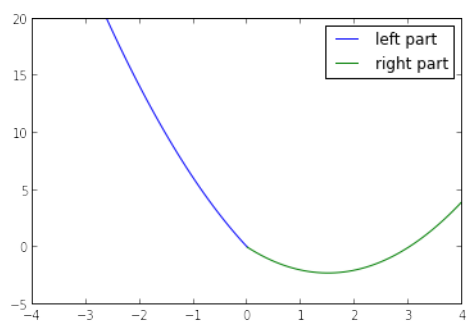
\includegraphics[height=1.3in]{fig/fig-han-1.PNG}
        \caption{$\tilde{x}^->0$, $\tilde{x}^+>0$, the minima is at $\tilde{x}^+$.}
    \end{subfigure}%
    ~
    \begin{subfigure}[t]{0.31\textwidth}
        \centering
        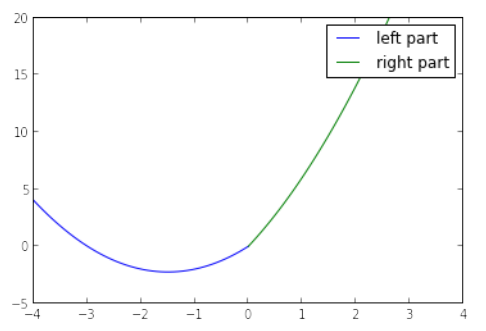
\includegraphics[height=1.3in]{fig/fig-han-2.PNG}
        \caption{$\tilde{x}^-<0$, $\tilde{x}^+<0$, the minima is at $\tilde{x}^-$.}
    \end{subfigure}
    ~
    \begin{subfigure}[t]{0.31\textwidth}
        \centering
        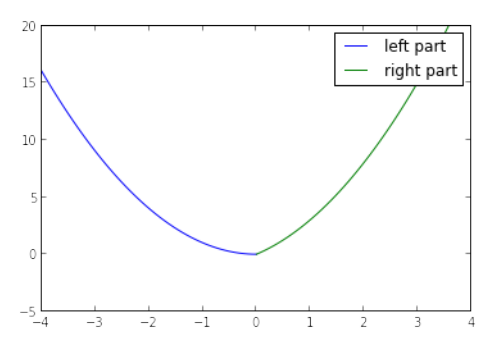
\includegraphics[height=1.3in]{fig/fig-han-3.PNG}
        \caption{$\tilde{x}^->0$, $\tilde{x}^+<0$, the minima is at 0.}
    \end{subfigure}
    \caption{Example picture of three cases.}
    \label{fig:hl1} 
\end{figure*}

\item {[}8 points{]} 
Write $x^*$, the minimum of $f_2(x)$, as a piecewise function of g. (Hint: what is
g in the cases above?)\\
\underline{\textbf{Answer:}}\\
Summarizing the result from the previous question, we have
\begin{equation}
x^*=
\begin{cases}
\tilde{x}^+ &\text{if $\tilde{x}^+>0$}\\
\tilde{x}^- &\text{if $\tilde{x}^-<0$}\\
0 &\text{if $\tilde{x}^+<0, \tilde{x}^->0$}
\end{cases}
\end{equation}
This is equivalent to the soft-threshold function
\begin{equation}
x^*=
\begin{cases}
   -\frac{g+\alpha}{h} &\text{if $g<-\alpha$}\\
   0 &\text{if $g\in\left[-\alpha, \alpha\right]$}\\
   -\frac{g-\alpha}{h} &\text{if $g>\alpha$}
   \end{cases}
\end{equation}

\item {[}8 points{]} 
Now let’s derive the update rule for $w_k$. Fixing all parameters but $w_k$, express the objective function in the form of Eq.~\eqref{eq:hl1} (here $w_k$ is our x). You do not
need to explicity write constant factors, you can put them all together as c. What are
g and h? Then putting it all together, write down the coordinate descent algorithm for the Elastic Net (\textbf{again excluding} $w_0$). You can write the update for $w_k$ in terms of the g and h you calculated in the previous question.\\
\underline{\textbf{Answer:}}\\
\begin{equation}
g=\sum^n_{j=1}x^{(j)}_k(\sum_{i\neq k}\vec{w}_i\vec{x}_i^{(j)}-y_i)
\end{equation}
\begin{equation}
h=\lambda+\sum^n_{j=1}(x^{(j)})^2
\end{equation}
The algorithm is shown in Algorithm.~\ref{algo:hl1}. You can compare it to the CD algorithm for Lasso, the only difference is adding $\lambda$ to h.\\
\begin{algorithm}[H]\label{algo:hl1}
\SetAlgoLined
% \KwResult{Write here the result }
%  initialization\;
 \While{not converged}{
  % instructions\;
  \For{$k\in \{1,2,\cdots,d\}$}{
   $g=\sum^n_{j=1}x^{(j)}_k(\sum_{i\neq k}\vec{w}_i\vec{x}_i^{(j)}-y_i)$\;
   $h=\lambda+\sum^n_{j=1}(x^{(j)})^2$\;
   $w_k=\begin{cases}
   -\frac{g+\alpha}{h} &\text{if $g<-\alpha$}\\
   0 &\text{if $g\in\left[-\alpha, \alpha\right]$}\\
   -\frac{g-\alpha}{h} &\text{if $g>\alpha$}
   \end{cases}$\;
   }{
   % instructions3\;
  }
 }
 \caption{Coordinate Descent for Elastic Net}
\end{algorithm}
\end{qparts}

\newpage
\section{True or False questions (HL)}
Answer True or False. Justify your answer very briefly in 1-2 sentences.
\begin{qparts}
\item Increasing the regularization parameter $\lambda$ in lasso regression leads to sparser regression coefficients.
\underline{\textbf{Answer:}}\\
True. Larger regularization parameter penalizes non-zero coefficients more, leading to
sparser solution.

\item In Lasso regression, can the regulariser increase the sparsity of the resulting solutions?\\
\underline{\textbf{Answer:}}\\
True, Lasso introduces the L1 norm penalty, so increasing the penalty will cause more and more of the parameters to be driven to zero. As seen in \cref{fig:hl2}, where the red contours are representing the error function and the solid blue areas the constraint regions for the parameters, in the Lasso case, the function is likely to hit the constraint region on one of the four corners. This will make a parameter equal with zero.
\begin{figure}[!htb]
    \centering
    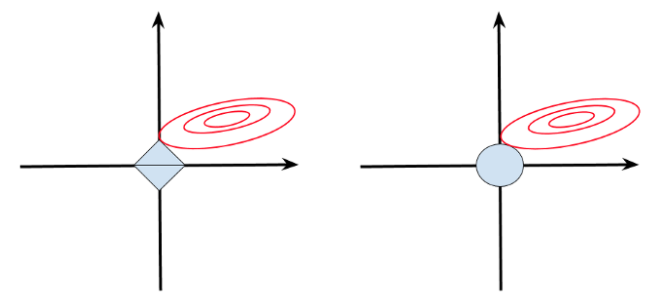
\includegraphics[width=.6\textwidth]{fig/fig-han-4.PNG}
    \caption{Spam-Estimation picture for the LASSO (left) and Ridge regression (right).}
    \label{fig:hl2}
\end{figure}

\item Is the objective of Lasso regression differentiable and convex?\\
\underline{\textbf{Answer:}}\\
False, it is not differentiable. As Lasso uses L1 norm penalty, this L1 loss function is defined based on the absolute value of the difference between two values. Since the loss function is a modulus function, there will exist an inflection point where the slope cannot be computed and the function is not differentiable. In contrast, for the case of Ridge regression, where we use L2 norm penalty, we can get the slope at any point and the objective is differentiable.

\item Are the objectives of Ridge and Lasso regression both convex and have closed-form solutions?\\
\underline{\textbf{Answer:}}\\
False, they are both convex, but Lasso does not always have a closed-form solution. LASSO regression must be solved numerically by using quadratic programming or more general convex optimisation methods.

\item Is it true that the L1 term in Lasso has the following purposes: performing feature selection, compensating for overfitting and smoothing?\\
\underline{\textbf{Answer:}}\\
False. The first two purposes are true, but not the last one. As it is mentioned early, both L1 and L2 terms are introduced to compensate for overfitting. By making the parameters equal with zero, the L1 norm discards some features and, thus, performs feature selection. In terms of smoothing, we cannot say L1 has this purpose, as the L1 loss function does not have continuous derivatives.
\end{qparts}
\end{document}